\documentclass[12pts, letterpaper]{article}

\usepackage[utf8]{inputenc}
\usepackage{amsmath}
\usepackage{amssymb}
\usepackage{amsthm}
\usepackage{amsfonts}
\usepackage{physics}
\usepackage{enumerate}
\usepackage{graphicx}
\graphicspath{ {images/} }
\usepackage[margin=1in]{geometry}
\usepackage{fancyhdr}
\usepackage{sectsty}
\subsubsectionfont{\centering}

\lhead{\sffamily{Quantum Information and Quantum Computation}}
\rhead{\sffamily{Vibhav Aggarwal}}
\cfoot{\sffamily{\thepage}}
\numberwithin{equation}{section}
\theoremstyle{definition}
\newtheorem{theorem}{Theorem}
\newtheorem{postulate}{Postulate}
\newtheorem{lemma}[theorem]{Lemma}
\newtheorem{corollary}[theorem]{Corollary}
\newtheorem{definition}{Definition}
\numberwithin{definition}{section}
\numberwithin{theorem}{section}
\newtheorem*{thesis}{Thesis}
\newtheorem{exercise}{Exercise}
\newtheorem*{example}{Example}

\theoremstyle{remark}
\numberwithin{exercise}{section}
\newtheorem*{solution}{Solution}
\pagestyle{fancy}

\setcounter{section}{-1}

\setlength\parindent{0pt}
\title{Quantum Information and Quantum Computation}
\author{Vibhav Aggarwal\thanks{Mentored by Neeraj Sohani}}
\date{April 2020}

\begin{document}

\maketitle

\tableofcontents
\newpage
\section{Introduction}

Quantum computation and quantum information is the study of the information processing tasks that can be accomplished using quantum mechanical systems. It is relatively a newer field of research and much work is going on to actually make a functional quantum computer. Big tech companies like Google, Microsoft, Hitachi, Mitsubishi, Nokia, etc. are investing huge amounts of money in research and development of quantum computers.
\vspace{1em}

But why? What is so special about this field that so many people are interested in it? Turns out, quantum computers offer an essential speed advantage over classical computers. This speed advantage is so significant that many researchers believe that no conceivable amount of progress in classical computation would be able to overcome the gap between the power of a classical computer and the power of a quantum computer!
\vspace{1em}

For example, the RSA cryptosystem used for transferring data in secure manner is just based on the fact that it is very difficult for a classical computer to factorize large numbers (order of 2048 bits) quickly. Till date there is simply no known algorithm to that efficiently on a classical computer. However, there is an algorithm known as Shor’s algorithm which can just do that really quickly on a quantum computer.
\vspace{1em}

There are many other algorithms based upon quantum computers and one class of such algorithms is the \textit{quantum search algorithms}. The quantum search algorithm solves
the following problem: Given a search space of size $N$, and no prior knowledge about the
structure of the information in it, we want to find an element of that search space satisfying a known property. How long does it take to find an element satisfying that property?
Classically, this problem requires approximately $N$ operations, but the quantum search algorithm allows it to be solved using approximately $\sqrt{N}$ operations.
\vspace{1em}

Another important use is \textit{quantum simulation}. Simulation of quantum systems on classical machines is difficult and the space requirement grows exponentially with increasing number of components in the system. But in case of quantum computers, this growth is linear and therefore they can be used in quantum chemistry to simulate large molecules and study the inter-atomic interactions.

\newpage
\section{Quantum bits (qubits)}

The \textit{bit} is the fundamental concept of classical computation. It has only two possible states: $0$ and $1$. Any information can be represented by a combination of bits. Using $n$ bits, a total of $2^n$ different messages can be represented/conveyed.
\\\\
Quantum computation and quantum information are built upon an analogous concept, the \textit{quantum bit}, or \textit{qubit} for short. Qubits are mathematical objects with certain properties. While it is true that qubits, like bits, are realized as actual physical systems, we are going to treat them as abstract mathematical objects.
\\\\
A qubit has a state, just like a bit, represent by $\ket{\psi}$. Two possible states are $\ket{0}$ and $\ket{1}$. However it can also have a state which is a linear combination of these two. Thus:
\begin{center}
    $\ket{\psi}=\alpha\ket{0} + \beta\ket{1}$
\end{center}

The numbers $\alpha$ and $\beta$ are complex numbers. Put another way, the state of a qubit is a vector in a two-dimensional complex vector space. The special states $\ket{0}$ and $\ket{1}$ are known as computational basis states, and form an \textit{orthonormal} basis for this vector space.
\\\\
Since $\alpha$ and $\beta$ can take infinitely many different complex values, one might be tempted to think that infinite different messages can be conveyed using a single qubit! But there's a catch. When we make a measurement of a qubit, its state \textit{collapses} into either $\ket{0}$ with probability $|\alpha|^2$ or $\ket{0}$ with probability $|\beta|^2$. So every time we observe only one of the two possible states. Naturally, $|\alpha|^2 + |\beta|^2 = 1$. 
\\\\
Geometrically, we can interpret this as the condition that the qubit’s state be normalized to length $1$. Thus, in general a qubit’s state is a unit vector in a two-dimensional complex vector space.
\\\\
Since $\alpha$ and $\beta$ are complex numbers with the only constraint that $|\alpha|^2 + |\beta|^2 = 1$, we may represent the state of qubit as:
    $$\ket{\psi} = e^{i\gamma}\left(\cos{\frac{\theta}{2}}\ket{0} + e^{i\phi}\sin{\frac{\theta}{2}}\ket{1}\right)$$

In fact, we can ignore the factor $e^{i\gamma}$ because it has no observable effects. Thus we can effectively write:
    $$\ket{\psi} = \cos{\frac{\theta}{2}}\ket{0} + e^{i\phi}\sin{\frac{\theta}{2}}\ket{1}$$

The numbers $\theta$ and $\phi$ define a point on the unit three-dimensional sphere, as shown in the figure below. This sphere is often called the \textit{Bloch sphere}.
\begin{figure}[h]
    \centering
    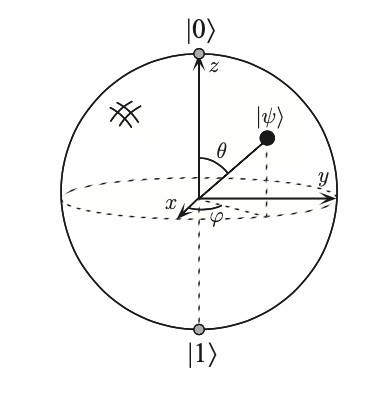
\includegraphics[width=0.35\textwidth]{bloch.png}
    \caption{Bloch sphere}
\end{figure}

\newpage
\section{Introduction to Quantum Mechanics}
To understand the concepts of quantum information and computing, a thorough understanding of quantum mechanics is required. Thus we must first get familiar with the mathematics involved and later we will see the postulates of quantum mechanics.

\subsection{Linear Algebra}
Linear algebra is the study of vector spaces and of linear operations on those vector spaces. A good understanding of quantum mechanics is based upon a solid grasp of elementary linear algebra.
\begin{definition}
    A \textit{spanning set} for a vector space is a set of vectors $\ket{v_1},\ldots,\ket{v_n}$ such that any vector $\ket{v}$ in the vector space can be written as a linear combination $\ket{v} = \sum_{i}{a_i\ket{v_i}}$ of vectors in that set. 
\end{definition}
\begin{definition}
    A \textit{linear operator} between vector spaces $V$ and $W$ is defined to be any function $A \colon\ V\ \rightarrow\ W$ which is linear in its inputs, $$A\left(\sum_{i}{a_i\ket{v_i}}\right)=\sum_{i}{a_iA\left(\ket{v_i}\right)}$$
\end{definition}
\\
The most convenient way to understand linear operators is in terms of their \textit{matrix representation}. Suppose $A \colon\ V\ \rightarrow\ W$ is a linear operator between vector spaces $V$ and $W$. Suppose $\ket{v_1},\ldots,\ket{v_m}$ is a basis for $V$ and $\ket{w_1},\ldots,\ket{w_n}$ is a basis for $W$ . Then for each $j$ in the range $1,\ldots,m$, there exist complex numbers $A_{1j}$ through $A_{nj}$ such that
    $$A\ket{v_j} = \sum_{i = 1}^{n}{A_{ij}\ket{w_i}}$$

The $n\times m$ matrix whose entries are the values $A_{ij}$ is said to form a matrix representation of the operator $A$.

Matrix representation is very helpful in the way that applying operator A to a vector $\ket{v}$ is equivalent to multiplying the matrix of $A$ by the column vector representation of $\ket{v}$.

\subsubsection*{The Pauli matrics}
Four extremely useful matrices are the Pauli matrices. They are defined as:
\begin{align*}
    \sigma_0\equiv\ I\equiv\begin{bmatrix}1&0\\0&1\\\end{bmatrix} && \sigma_1\equiv\sigma_x\equiv\ X\equiv\begin{bmatrix}0&1\\1&0\\\end{bmatrix}\\
    \sigma_2\equiv\sigma_y\equiv\ Y\equiv\begin{bmatrix}0&-i\\-i&0\\\end{bmatrix} && \sigma_3\equiv\sigma_z\equiv\ Z\equiv\begin{bmatrix}1&0\\0&-1\\\end{bmatrix}
\end{align*}

\subsubsection{Inner Products}
An \textit{inner product} is a function which takes as input two vectors $\ket{v}$ and $\ket{w}$ from a vector space and produces a complex number as output. For the time being, it will be convenient to write the inner product of $\ket{v}$ and $\ket{w}$ as $\left(\ket{v}, \ket{w}\right)$ although the standard quantum mechanical notation is $\braket{v}{w}$.
\\\\
A function $(\cdot, \cdot)$ from $V \cross V$ to $C$ is an inner product if it satisfies the requirements that:
\begin{enumerate}
    \item $(\cdot, \cdot)$ is linear in the second argument,
        $$\left(\ket{v}, \sum_{i}{\lambda_i\ket{w_i}}\right) = \sum_{i}{\lambda_i\left(\ket{v}, \ket{w_i}\right)}$$
    \item $\left(\ket{v}, \ket{w}\right) = \left(\ket{w}, \ket{v}\right)^\ast$
    \item $\left(\ket{v}, \ket{v}\right) \geq 0$ with equality if and only if $\ket{v} = 0$
\end{enumerate}

A vector space having an inner product is called an \textit{inner product space}.

For example, $\mathbb{C}^n$ has an inner product defined by
    $$((y_1,\ldots,y_n), (z_1,\ldots,\z_n)) = \sum_{i}{y_i^\ast z_i} = \begin{bmatrix}y_1^\ast & \dots & y_n^\ast\end{bmatrix} \begin{bmatrix}z_1 \\ \vdots \\ z_n\end{bmatrix}$$
\\\\
In the finite dimensional complex vector spaces that come up in quantum computation and quantum information, a \textit{Hilbert space} is \textit{exactly the same thing} as an inner product space. From now on we may use the two terms interchangeably.
\\\\
\begin{definition}
    Vectors $\ket{v}$ and $\ket{w}$ are \textit{orthogonal} if their inner product is zero.
\end{definition}
\begin{definition}
    The \textit{norm} of a vector is defined as,
        $$\norm{\ket{v}} = \sqrt{\braket{v}{v}}$$
\end{definition}
\begin{definition}
    A \textit{unit vector} is a vector $\ket{v}$ such that $\norm{\ket{v}} = 1$.
\end{definition}

\subsubsection{Eigenvectors and eigenvalues}
\begin{definition}
    An \textit{eigenvector} of a linear operator $A$ on a vector space is a non-zero vector $\ket{v}$ such that $A\ket{v} = v\ket{v}$, where $v$ is a complex number known as the \textit{eigenvalue} of $A$ corresponding to $\ket{v}$.
\end{definition}
\begin{definition}
    A \textit{diagonal representation} for an operator $A$ on a vector space $V$ is a representation $A = \sum_{i}{\lambda_i\ket{i}\bra{i}}$, where the vectors $\ket{i}$. form an orthonormal set of eigenvectors for $A$, with corresponding eigenvalues $\lambda_i$. Diagonal representations are sometimes also known as \textit{orthonormal decompositions}.
\end{definition}
\begin{definition}
    An operator is said to be \textit{diagonalizable} if it has a diagonal representation.
\end{definition}

\subsubsection{Adjoint and Hermitian operators}
\begin{definition}
    Suppose $A$ is any linear operator on a Hilbert space, $V$. There exists a unique operator $A^\dag$ on $V$ such that for all vectors $\ket{v}, \ket{w}\in V$, $(\ket{v}, A\ket{w}) = (A^\dag\ket{v}, \ket{w})$. The linear operator $A^\dag$ is known as the \textit{adjoint} or \textit{Hermitian conjugate} of the operator A.
\end{definition}
It can be proved that $A^\dag = (A^\ast)^T$
\begin{definition}
    An operator $A$ is said to be \textit{normal} if $AA^\dag=A^\dag A$.
\end{definition}
\begin{definition}
    An operator $A$ is said to be \textit{unitary} if $AA^\dag=\ I$.
\end{definition}
\begin{theorem}
    \textbf{(Spectral decomposition)} Any normal operator $M$ on a vector space $V$ is diagonal with respect to some orthonormal basis for $V$. Conversely, any diagonalizable operator is normal.
\end{theorem}
\begin{exercise}
    Show that a normal matrix is Hermitian if and only if it has real eigenvalues.
\end{exercise}
\begin{solution}
    $\left(\Longrightarrow\right)\tab$ Let $A\ket{v} = \lambda\ket{v}$. We have,
    \begin{equation*}
    \begin{split}
        (\ket{v}, A\ket{V}) & = (A^\dag\ket{v}, \ket{v}) \\
        (\ket{v}, \lambda\ket{v}) & = (\lambda\ket{v}, \ket{v}) \\
        \lambda(\ket{v}, \ket{v}) & = \lambda^*(\ket{v}, \ket{v}) \\
        \lambda & = \lambda^*
    \end{split}
    \end{equation*}
    
    $\left(\Longleftarrow\right)\tab$ By the spectral theorem, if $A$ is normal, then it is diagonalizable. Hence, $A=UDU^\dag$ for some unitary operator matrix $U$ and a diagonal matrix $D$ containing eigenvalues of $A$. Taking adjoint on both sides,
    \begin{equation*}
    \begin{split}
        A^\dag & = \left(UDU^\dag\right)^\dag \\
        & = UD^\ast U^\dag \\
        & = UDU^\dag \\
        & = A
    \end{split}
    \end{equation*}
\end{solution}

\begin{exercise}
    Show that all eigenvalues of a unitary matrix have modulus $1$, that is, can be written in the form $e^{i\theta}$ for some real $\theta$.
\end{exercise}
\begin{solution}
    \begin{equation*}
    \begin{split}
        U\ket{v} & = \lambda\ket{v} \\
        \implies \bra{v}U^\dag & = \bra{v}\lambda^\ast
    \end{split}
    \end{equation*}
    By multiplying the above equations, we get
    \begin{equation*}
    \begin{split}
        \bra{v}U^\dag U\ket{v} & = \bra{v}\lambda^\ast\lambda\ket{v} \\
        \braket{v}{v} & = \norm{\lambda}^2\braket{v}{v} \\
        \norm{\lambda}^2 & = 1 \\
        \norm{\lambda} & = 1
    \end{split}
    \end{equation*}
\end{solution}

\begin{definition}
    A positive operator $A$ is defined to be an operator such that for any vector $\ket{v}$, $(\ket{v}, A\ket{v})$ is a real, non-negative number.
\end{definition}

\begin{exercise}
    Show that a positive operator is necessarily Hermitian.
\end{exercise}
\begin{solution}
    Let
    \begin{align*}
        B = \frac{A+A^\dag}{2} && C = \frac{-iA+iA^\dag}{2}
    \end{align*}
    Then $B$ and $C$ are Hermitian and $A = B + iC$
    Hence
    $$\bra{v}A\ket{v} = \bra{v}B\ket{v} + i\bra{v}C\ket{v}$$
    Any Hermitian $X$ can be represent as $X = \sum_{i}{\lambda_i\ket{i}\bra{i}}$ where $\ket{i}$ are its eigenvectors and $\lambda_i$ are corresponding eigenvalues.
    For any vector $\ket{v}$, $\bra{v}X\ket{v} = \sum_{i}{\lambda_i\braket{v}{i}\braket{i}{v}}$ which is always real.
    Hence $\bra{v}C\ket{v} = 0$ for all vectors $\ket{v}$ and this combined with the fact that $C$ is Hermitian yields that $C$ is identically $0$. Therefore, $A$ must be Hermitian.
\end{solution}

\subsubsection{Tensor products}
The \textit{tensor product} is a way of putting vector spaces together to form larger vector spaces. This construction is crucial to understanding the quantum mechanics of multiparticle systems.
\\\\
In layman terms, tensor product of two vectors \textit{from different vector spaces} is simply the "concatenation" of these vectors (i.e. placing next to each other).
\\\\
Suppose $V$ and $W$ are vector spaces of dimension $m$ and $n$ respectively. For convenience we also suppose that $V$ and $W$ are Hilbert spaces. Then $V \otimes W$ (read '$V$ tensor $W$') is an $mn$ dimensional vector space. The elements of $V \otimes W$ are linear combinations of 'tensor products' $\ket{v}\otimes\ket{w}$ of elements $\ket{v}$ of $V$ and $\ket{w}$ of $W$. In particular, if $\ket{i}$ and $\ket{j}$ are orthonormal bases for the spaces $V$ and $W$ then $\ket{i}\otimes\ket{j}$ is a basis for $V \otimes W$.
\\\\
Tensor product can be defined for operators too. Let $A$ and $B$ be linear operators acting on vector spaces $V$ and $W$ respectively. Then the operator $A \otimes B$ acting on $V \otimes W$ is defined as
    $$(A \otimes B)(\ket{v}\otimes\ket{w}) \equiv (A\ket{v})\otimes(B\ket{w})$$

The inner products on the spaces $V$ and $W$ can be used to define a natural inner product on $V \otimes W$ . Define
    $$\left(\sum_{i}{a_i\ket{v_i}\otimes\ket{w_i}}, \sum_{j}{b_j\ket{v_j'}\otimes\ket{w_j'}}\right) \equiv = \sum_{ij}{a_i^\ast b_j\braket{v_i}{v_j'}\braket{w_i}{w_j'}}$$
It can be shown that the function so defined is a well-defined inner product.
\\\\
Now we discuss the \textit{Kroneckar product} which is a convenient matrix representation of $A \otimes B$. Suppose $A$ is an $m \cross n$ matrix, and $B$ is a $p \cross q$ matrix. Then we have the matrix representation:
    $$A \otimes B = \overbrace{\left.\begin{bmatrix}
                                A_{11}B & A_{12}B & \dots & A_{1n}B \\
                                A_{21}B & A_{22}B & \dots & A_{2n}B \\
                                \vdots & \vdots & \ddots & \vdots \\
                                A_{m1}B & A_{m2}B & \dots & A_{mn}B \\
                                \end{bmatrix}\right\}}^{nq}mp$$

We use $\ket{\psi}^{\otimes k}$ to denote $\ket{\psi}$ tensored with itself $k$ times.

\subsubsection{Operator functions}
There are many important functions which can be defined for operators and matrices. Generally speaking, given a function $f$ from the complex numbers to the complex numbers, it is possible to define a corresponding matrix function on normal matrices by the following construction. Let A = $\sum_{a}{a\ket{a}\bra{a}}$ be a spectral decomposition for a normal operator $A$. Define $f(A) \equiv \sum_{a}{f(a)\ket{a}\bra{a}}$. This procedure can be used, for example, to define the square root of a positive operator, the logarithm of a positive-definite operator, or the exponential of a normal operator.
\begin{exercise}
    \textbf{(Exponential of the Pauli matrices)} Let $\vec{v}$ be any real, three-dimensional unit vector and $\theta$ a real number. Prove that
        $$\exp\left(i\theta\vec{v}\cdot\vec{\sigma}\right) = \cos(\theta)I + i\sin(\theta)\vec{v}\cdot\vec{\sigma},$$
    where $\vec{v}\cdot\vec{\sigma} = \sum_{i = 1}^{3}v_i\sigma_i$.
\end{exercise}
\begin{solution}
    Note that $\sigma_i\sigma_j = \left\{
                        \begin{matrix}
                            I, & if\ i = j \\ 
                            -\sigma_j\sigma_i, & if\ i \neq j
                        \end{matrix}\right.$
    \\\\Hence, $(\vec{v}\cdot\vec{\sigma})^2 = (v_1^2 + v_2^2 + v_3^2)I = I$
    \begin{equation*}
    \begin{split}
        \exp\left(i\theta\vec{v}\cdot\vec{\sigma}\right) & = \sum_{k = 0}^{\infty}{\frac{(i\theta\vec{v}\cdot\vec{\sigma})^k}{k!}} \\
        & = \sum_{k = 0}^{\infty}{\frac{(i\theta\vec{v}\cdot\vec{\sigma})^{2k}}{(2k)!}} + \sum_{k = 0}^{\infty}{\frac{(i\theta\vec{v}\cdot\vec{\sigma})^{2k+1}}{(2k+1)!}} \\
        & = \sum_{k = 0}^{\infty}{\frac{(-1)^k(\theta)^{2k}I}{(2k)!}} + i\vec{v}\cdot\vec{\sigma}\sum_{k = 0}^{\infty}{\frac{(-1)^k(\theta)^{2k+1}}{(2k+1)!}} \\
        & = \cos(\theta)I + i\sin(\theta)\vec{v}\cdot\vec{\sigma}
    \end{split}
    \end{equation*}
\end{solution}
\vspace{1em}

An important matrix function is the \textit{trace} of a matrix.
\begin{definition}
    The trace of A is defined to be the sum of its diagonal elements,
    $$tr(A) \equiv \sum_{i}{A_{ii}}$$
\end{definition}
The following properties can easily be proved for the trace of a matrix:
\begin{enumerate}
    \item $\tr(AB) = \tr(BA)$
    \item $\tr(A + B) = \tr(A) + \tr(B)$
    \item $\tr(zA) = z\tr(A)$
\end{enumerate}

\subsubsection{The commutator and anti-commutator}
\begin{definition}
    The \textit{commutator} between two operators A and B is defined to be
    $$[A, B] = AB - BA$$
\end{definition}
\begin{definition}
    The \textit{anti-commutator} between two operators A and B is defined to be
    $$\{A, B\} = AB + BA$$
\end{definition}
If $[A, B] = 0$, we say that $A$ \textit{commutes} with $B$. Similarly, If ${A, B} = 0$, we say that $A$ \textit{ant-commutes} with $B$.
\begin{theorem}
    \textbf{(Simultaneous diagonalization theorem)} Suppose $A$ and $B$ are Hermitian operators. Then $[A, B] = 0$ if and only if there exists an orthonormal basis such that both $A$ and $B$ are diagonal with respect to that basis. We say that $A$ and $B$ are \textit{simultaneously diagonalizable} in this case.
\end{theorem}
\begin{proof}
    It can be easily verified that if $A$ and $B$ are diagonal in the same orthonormal basis then $[A,B] = 0$. To show the converse, let $\ket{a, j}$ be an orthonormal basis for the eigenspace $V_a$ of $A$ with eigenvalue $a$; the index $j$ is used to label possible degeneracies. Note that
        $$AB\ket{a, j} = BA\ket{a, j} = aB\ket{a, j}$$
    and therefore $B\ket{a, j}$ is an element of the eigenspace $V_a$. Let $P_a$ denote the projector onto the space $V_a$ and define $B_a \equiv P_aBP_a$. It is easy to see that the restriction of $B_a$ to the space $V_a$ is Hermitian on $V_a$, and therefore has a spectral decomposition in terms of an orthonormal set of eigenvectors which span the space $V_a$. Let’s call these eigenvectors $\ket{a, b, k}$, where the indices $a$ and $b$ label the eigenvalues of $A$ and $B_a$, and $k$ is an extra index to allow for the possibility of a degenerate $B_a$. Note that $B\ket{a, b, k}$ is an element of $V_a$, so $B\ket{a, b, k} = P_aB\ket{a, b, k}$. Moreover we have $P_a\ket{a, b, k} = \ket{a, b, k}$, so
        $$B\ket{a, b, k} = P_aBP_a\ket{a, b, k} = b\ket{a, b, k}$$
    It follows that $\ket{a, b, k}$ is an eigenvector of $B$ with eigenvalue $b$, and therefore $\ket{a, b, k}$ is an orthonormal set of eigenvectors of both $A$ and $B$, spanning the entire vector space on which $A$ and $B$ are defined. That is, $A$ and $B$ are simultaneously diagonalizable.
\end{proof}
\newpage
\subsubsection{The polar and singular value decompositions}
The \textit{polar} and \textit{singular value} decompositions are useful ways of breaking linear operators up into simpler parts. In particular, these decompositions allow us to break general linear operators up into products of unitary operators and positive operators. While we don’t understand the structure of general linear operators terribly well, we do understand unitary operators and positive operators in quite some detail. The polar and singular value decompositions allow us to apply this understanding to better understand general linear operators.
\begin{theorem}
    \textbf{(Polar decomposition)} Let $A$ be a linear operator on a vector space $V$. Then there exists unitary $U$ and positive operators $J$ and $K$ such that
    $$A = UJ = KU,$$
    where the unique positive operators $J$ and $K$ satisfying these equations are defined by $J \equiv \sqrt{A^\dag A}$ and $K \equiv \sqrt{AA^\dag}$. Moreover,if $A$ is invertible then $U$ is unique.
\end{theorem}
\begin{corollary}
    \textbf{(Singular value decomposition)} Let $A$ be a square matrix. Then there exist unitary matrices $U$ and $V$, and a diagonal matrix $D$ with non-negative entries such that
        $$A = UDV$$
    The diagonal elements of $D$ are called the singular values of $A$.
\end{corollary}

\subsection{The postulates of quantum mechanics}
Quantum mechanics is a mathematical framework for the development of physical theories. On its own quantum mechanics doesn’t tell you what laws a physical system must obey, but it does provide a mathematical and conceptual framework for the development of such laws. In the next few sections we give a complete description of the basic postulates of quantum mechanics. These postulates provide a connection between the physical world and the mathematical formalism of quantum mechanics.

\subsubsection{State space}
\begin{postulate}
    Associated to any isolated physical system is a complex vector space with inner product (that is, a Hilbert space) known as the \textit{state space} of the system. The system is completely described by its \textit{state vector}, which is a unit vector in the system’s state space.
\end{postulate}
Quantum mechanics does \textit{not} tell us, for a given physical system, what the state space of that system is, nor does it tell us what the state vector of the system is. Figuring that out for a \textit{specific} system is a difficult problem for which physicists have developed many intricate and beautiful rules.
\\\\
The simplest quantum mechanical system, and the system which we will be most concerned with, is the \textit{qubit}. A qubit has a two-dimensional state space. Suppose $\ket{0}$ and $\ket{1}$ form an orthonormal basis for that state space. Then an arbitrary state vector in the state space can be written
    $$\ket{\psi} = a\ket{0} + b\ket{1}$$
 where $a$ and $b$ are complex numbers. The condition that $\ket{\psi}$ be a unit vector, $\braket{\psi}{\psi} = 1$, is therefore equivalent to $|a|^2 + |b|^2 = 1$. The condition $\braket{\psi}{\psi} = 1$ is often known as the \textit{normalization condition} for state vectors.
 
 \subsubsection{Evolution}
 How does the state, $\ket{\psi}$, of a quantum mechanical system change with time? The following postulate gives a prescription for the description of such state changes.
 \begin{postulate}
     The evolution of a \textit{closed} quantum system is described by a \textit{unitary transformation}. That is, the state $\ket{\psi}$ of the system at time $t_1$ is related to the state $\ket{\psi'}$ of the system at time $t_2$ by a unitary operator $U$ which depends only on the times $t_1$ and $t_2$,
        $$\ket{\psi'} = U\ket{\psi}$$
 \end{postulate}
 Just as quantum mechanics does not tell us the state space or quantum state of a \textit{particular} quantum system, it does not tell us which unitary operators $U$ describe real world quantum dynamics. Quantum mechanics merely assures us that the evolution of any closed quantum system may be described in such a way. An obvious question to ask is: what unitary operators are natural to consider? In the case of single qubits, it turns out that \textit{any} unitary operator at all can be realized in realistic systems.
 
 \subsubsection{Quantum measurement}
 We postulated that closed quantum systems evolve according to unitary evolution. The evolution of systems which don’t interact with the rest of the world is all very well, but there must also be times when the experimentalist and their experimental equipment – an external physical system in other words – observes the system to find out what is going on inside the system, an interaction which makes the system no longer closed, and thus not necessarily subject to unitary evolution. To explain what happens when this is done, we introduce Postulate 3, which provides a means for describing the effects of measurements on quantum systems.
\begin{postulate}
    Quantum measurements are described by a collection $\{M_m\}$ of measurement operators. These are operators acting on the state space of the system being measured. The index $m$ refers to the measurement outcomes that may occur in the experiment. If the state of the quantum system is $\ket{\psi}$ immediately before the measurement then the probability that result $m$ occurs is given by
        $$p(m) = \bra{\psi}M_m^\dag M_m\ket{\psi} ,$$
    and the state of the system after the measurement is
    $$\frac{M_m\ket{\psi}}{\sqrt{\bra{\psi}M_m^\dag M_m\ket{\psi}}}$$
    The measurement operators satisfy the \textit{completeness equation},
        $$\sum_{m}{M_m^\dag M_m} = I$$
  
    The completeness equation expresses the fact that probabilities sum to one:
        $$1 = \sum_{m}{p(m)} = \sum_{m}{\bra{\psi}M_m^\dag M_m\ket{\psi}}$$
\end{postulate}

A simple but important example of a measurement is the \textit{measurement of a qubit in the computational basis}. This is a measurement on a single qubit with two outcomes defined by the two measurement operators $M_0 = \ket{0}\bra{0}$, $M_1 = \ket{1}\bra{1}$. Observe that each measurement operator is Hermitian, and that $M_0^2 = M_0$ , $M_1^2 = M_1$ . Thus the completeness relation is obeyed, $I = M_0^\dag M_0 + M_1^\dag M_1 = M_0 + M_1$. Suppose the state being measured is $\ket{\psi} = a\ket{0} + b\ket{1}$. Then the probability of obtaining measurement outcome $0$ is
    $$p(0) = \bra{\psi}M_0^\dag M_0\ket{\psi} = \bra{\psi}M_0\ket{\psi} = |a|^2$$
Similarly, the probability of obtaining the measurement outcome $1$ is $p(1) = |b|^2$. The
state after measurement in the two cases is therefore
    $$\frac{M_0\ket{\psi}}{|a|} = \frac{a}{|a|}\ket{0}$$
    $$\frac{M_1\ket{\psi}}{|b|} = \frac{b}{|b|}\ket{1}$$
The multipliers like $a/|a|$, which have modulus one, can effectively be ignored because they don't have any observable effect, so the two post-measurement states are effectively $\ket{0}$ and $\ket{1}$.

\subsubsection{Composite systems}
\begin{postulate}
    The state space of a composite physical system is the tensor product of the state spaces of the component physical systems. Moreover, if we have systems numbered $1$ through $n$, and system number $i$ is prepared in the state $\ket{\psi_i}$, then the joint state of the total system is $\ket{\psi_1}\otimes\ket{\psi_2}\otimes\ldots\otimes\ket{\psi_n}$
\end{postulate}

\begin{exercise}
    Show that the average value of the observable $X_1Z_2$ for a two qubit system measured in the state $(\ket{00} + \ket{11})/2$ is zero.
\end{exercise}
\begin{solution}
    Let $\ket{\psi} = \frac{\ket{00} + \ket{11}}{\sqrt{2}}$
    \\The average value of operator $X_1Z_2$ is given by $\bra{\psi}X_1Z_2\ket{\psi}$
    \begin{equation*}
    \begin{split}
        \bra{\psi}X_1Z_2\ket{\psi} & = \bra{\psi}X_1\left(\frac{\ket{00} - \ket{11}}{\sqrt{2}}\right) \\
        & = \left(\frac{\bra{00} + \bra{11}}{\sqrt{2}}\right)\left(\frac{\ket{10} - \ket{01}}{\sqrt{2}}\right) \\
        & = \frac{1}{2}\left(\braket{00}{10} - \braket{00}{01} + \braket{11}{10} - \braket{11}{01}\right) \\
        & = 0
    \end{split}
    \end{equation*}
    (since the four states $\ket{00}, \ket{01}, \ket{10}, \ket{11}$ are orthogonal)
\end{solution}
\vspace{1em}

Postulate 4 also enables us to define one of the most interesting and puzzling ideas associated with composite quantum systems – \textit{entanglement}.
\vspace{1em}

Formally, any multiple qubit state which cannot be factorized into single qubit states is called an \textit{entangled state}.
\vspace{1em}

For example, consider the state $\ket{\psi} = \frac{\ket{00} + \ket{11}}{\sqrt{2}}$. We are now going to show that it is entangled by contradiction.
\vspace{1em}

Let $\ket{\psi} = \ket{a}\ket{b}$, where $\ket{a}$ and $\ket{b}$ are single qubit states.
Further let $\ket{a} = \alpha_1\ket{0} + \beta_1\ket{1}$ and $\ket{b} = \alpha_2\ket{0} + \beta_2\ket{1}$.
Then,
    $$\frac{\ket{00} + \ket{11}}{\sqrt{2}} = \ket{\psi} = \ket{a}\ket{b} = \alpha_1\alpha_2\ket{00} + \alpha_1\beta_2\ket{01} + \beta_1\alpha_2\ket{10} + \beta_1\beta_2\ket{11}$$
Therefore, we have,
    $$\alpha_1\alpha_2 = \frac{1}{\sqrt{2}},$$
    $$\alpha_1\beta_2 = 0,$$
    $$\beta_1\alpha_2 = 0,$$
    $$\beta_1\beta_2 = \frac{1}{\sqrt{2}}$$
By multiplying first and fourth equations and second and third equations, we get two different values for the product $\alpha_1\alpha_2\beta_1\beta_2$ which is clearly a contradiction. Hence, the given state is entangled.
\vspace{1em}
% \newpage
% \section{Revised Plan of Action}
\begin{center}
\begin{tabular}{c|c}
    Week 4 & Density operator, EPR and Bell Inequality, models for computation \\
    Week 5 & Composite quantum systems, quantum circuits \\
    Week 6 & Quantum Fourier Transform and its applications \\
    Week 7 & Distance measures for quantum information
\end{tabular}
\end{center}
\end{document}
